\documentclass[11pt, a4paper]{article}

% --- PACKAGES ---
\usepackage[utf8]{inputenc}
\usepackage[T1]{fontenc}
\usepackage[english]{babel}
\usepackage{lmodern}
\usepackage{microtype}
\usepackage{graphicx}
\usepackage{amsmath, amssymb}
\usepackage{hyperref}
\usepackage{geometry}
\geometry{margin=2.4cm}
\usepackage{booktabs}
\usepackage{tabularx}
\usepackage{array}
\usepackage{enumitem}
\usepackage{caption}
\usepackage{float}
\usepackage{etoolbox}
\usepackage{xurl}

% --- LAYOUT & SECTION RULE ---
% Every top-level section starts on a new page (and flushes pending floats).
\preto\section{\clearpage}

% --- HYPERREF CONFIG ---
\hypersetup{
    colorlinks=true,
    linkcolor=black,
    urlcolor=blue,
    citecolor=black,
    pdftitle={100m Freestyle Swimming: Swimmer Profiling and Performance Modelling},
    pdfauthor={Paul-Emile Razafindrakoto}
}
\setlength{\parskip}{6pt}
\setlist{itemsep=3pt, topsep=3pt}

\begin{document}

% ============================================================
% COVER PAGE
% ============================================================
\begin{titlepage}
    \centering

    % --- Logos ---
    \vspace*{0.5cm}
    \begin{minipage}{0.35\textwidth}
        \centering
        
\includegraphics[height=2.2cm]{olympics.png}
    \end{minipage}
    \hfill
    \begin{minipage}{0.35\textwidth}
        \centering
        
\includegraphics[height=2.2cm]{world_aquatics.png}
    \end{minipage}

    \vspace{0.6cm}
    \rule{\textwidth}{0.4pt}
    \vspace{0.4cm}

    % --- Surtitle ---
    {\large\scshape Data Analysis \& Statistical Modelling Report\par}

    \vspace{0.4cm}

    % --- Main Title ---
    {\fontsize{28}{34}\bfseries 100m Freestyle Swimming\par}
    {\fontsize{20}{26}\bfseries Swimmer Profiling \& Performance Modelling\par}

    \vspace{0.35cm}

    {\large\textit{Characterizing top 100\,m Freestyle swimmers and predicting times from neighbouring events}\par}

    \vspace{0.4cm}
    \rule{\textwidth}{0.4pt}
    \vspace{0.6cm}

    % --- Abstract ---
    \begin{minipage}{0.86\textwidth}
        \small
        \textbf{Abstract.}
        This report studies how to characterize the profiles of top 100\,m Freestyle swimmers and model their performances from neighbouring events. Using World Aquatics Top~200 records and Olympic Games results (1912--2020), we combine Principal Component Analysis (SVD) to identify sprint profiles with linear regression and Ridge regularization to predict 100\,m times under collinearity.
    \end{minipage}

    \vfill

    % --- Author & Metadata ---
    {\small\textbf{Author}\\[4pt]}
    {\normalsize Paul-Emile RAZAFINDRAKOTO\par}

    \vspace{0.35cm}

    {\footnotesize Code repository: \href{https://github.com/perazaf1/swimming-analysis-acp}{github.com/perazaf1/swimming-analysis-acp}\par}
    {\footnotesize Data sources: World Aquatics Top~200 Records \& Olympic Swimming (1912--2020)\par}

    \vspace{0.3cm}

\end{titlepage}

% ============================================================
% CONTENTS
% ============================================================
\tableofcontents

\vspace{1.2cm}
\noindent\textit{Upcoming sections (in progress): Section~3 will cover 100\,m performance modelling under collinearity (OLS vs.\ Moore--Penrose vs.\ Ridge and 2D Fisher confidence ellipsoids), followed by Section~4 on limitations and extensions.}

% ============================================================
% USE OF ARTIFICIAL INTELLIGENCE
% ============================================================
\section*{Use of Artificial Intelligence}
\addcontentsline{toc}{section}{Use of Artificial Intelligence}

This project is an independent personal study written for publication. For transparency, this section details how AI tools were used alongside the author's own work and verification steps.

\subsection*{Models Used}
\begin{itemize}
    \item \textbf{Gemini 4 Argon:} used for Python code development (data cleaning and PCA/SVD scripts), code review, and checking schema and value consistency across the CSV datasets.

    \item \textbf{Gemini 4 Hydrogen:} used for drafting assistance, \LaTeX{} typesetting, and document compilation.

    \item \textbf{Deepseek V4.1 Pro:} used to review the mathematical formulations and keep notations consistent across the linear algebra and statistics sections.
\end{itemize}

\subsection*{Author Responsibility, Verification, and Reproducibility}
\begin{itemize}
    \item \textbf{Author role and editorial control:} the research question, data selection choices (including the 1988 Olympic cutoff and gender-wise standardization), sporting interpretations, and final wording of every section were decided and reviewed by the author, who takes full responsibility for the content and any remaining errors.

    \item \textbf{No AI-generated figures or numbers:} no numerical results, tables, or plots were produced or estimated by a language model. Every number in this report comes directly from local Python scripts executed on the raw World Aquatics and Olympic datasets.

    \item \textbf{Verification protocol:} all scripts include automated consistency checks covering table shapes, missing-value counts, and linear algebra identities (such as $V^T V = I_r$ and Eckart--Young reconstruction errors verified to machine precision $< 10^{-10}$). Generated plots and compiled PDF pages were inspected visually.

    \item \textbf{Open reproducibility:} all Python scripts and \LaTeX{} sources are published on GitHub (\url{https://github.com/perazaf1/swimming-analysis-acp}) so every result can be reproduced independently without relying on any AI tool.
\end{itemize}

% ============================================================
% SECTION 1: INTRODUCTION & DATA PIPELINE
% ============================================================
\section{Introduction \& Data Pipeline}
\label{sec:intro}

\subsection{Context \& Research Question}

The 100\,m Freestyle (50\,m long-course pool) is one of the most competitive events in swimming. At the elite level, a race lasts around 46 to 55 seconds and relies on two main physical qualities:
\begin{itemize}
    \item \textbf{Pure sprint power}, needed for the start and the first 50\,m (shared with the 50\,m Freestyle);
    \item \textbf{Speed endurance}, needed to maintain pace over the second half of the race despite fatigue (shared with the 200\,m Freestyle and 100\,m Butterfly).
\end{itemize}

\noindent Because swimmers lean toward either pure speed or endurance, looking at their times across several events tells us a lot about their profile. This leads to the main question of this report:
\begin{quote}
    \textbf{\textit{How can we characterize the profiles of top 100\,m Freestyle swimmers and model their performances from neighbouring events?}}
\end{quote}

\noindent \textbf{Implementation choice:} rather than using high-level machine learning Python packages such as \texttt{scikit-learn}, all dimensionality reduction, missing-data completion, and regression estimators are implemented directly from linear algebra primitives in \texttt{NumPy} and \texttt{SciPy} (alongside \texttt{pandas} for cleaning). This deliberate choice avoids black-box defaults and keeps a direct link between the mathematical derivations and every numerical result reported here.

\subsection{Raw Datasets}

We combine two complementary datasets:
\begin{enumerate}
    \item \textbf{World Aquatics All-Time Top~200~\cite{kaggle_top200}:} 5{,}200 long-course performances covering the 200 fastest historical times across 26 categories (13 men's and 13 women's events, 100\,m to 1500\,m) between 1980 and 2022, for 716 unique athletes. An important limitation is that \textbf{the 50\,m Freestyle is absent} from this file (distances start at 100\,m).

    \item \textbf{Olympic Games Swimming Results (1912--2020)~\cite{kaggle_olympics}:} 4{,}359 Olympic entries spanning 1912 to 2020, including relays and non-finishing entries. Unlike the Top~200 dataset, it contains the \textbf{50\,m Freestyle}, which makes it essential to link pure sprint speed with the 100\,m Freestyle.
\end{enumerate}

\subsection{Data Cleaning}

Both raw files are cleaned and harmonized in Python using reproducible rules:
\begin{itemize}
    \item \textbf{Time conversion:} mixed string formats (\texttt{"46.86"}, \texttt{"01:45.30"}, \texttt{"00:01:00.000000"}, and estimated times ending in \texttt{"est"}) are converted to decimal seconds. Disqualified, empty, and missing entries map to \texttt{NaN}.

    \item \textbf{Dates and age:} two-digit \texttt{MM-DD-YY} dates are parsed with a 2025 century pivot to recover true dates between 1980 and 2022. Athlete age is computed as $(\text{swim date} - \text{birth date}) / 365.25$, ranging from 13.98 to 34.32 years (median 22.70).

    \item \textbf{Name and event normalization:} \texttt{"LAST, First"} strings are unified to \texttt{"First Last"}, and event labels are standardized across both datasets (e.g.\ \texttt{"200m Individual Medley"}).

    \item \textbf{Olympic filtering:} from 4{,}359 raw Olympic rows, we keep individual events (3{,}619 rows) with valid times (3{,}511 rows) from \textbf{1988 to 2020} (when the 50\,m Freestyle became a permanent Olympic event), and remove duplicates, leaving \textbf{1{,}869} clean records across 960 athletes (943 Men, 926 Women; zero missing values).
\end{itemize}

\subsection{Processed Tables \& Limitations}

The cleaning step produces four analysis tables summarized in Table~\ref{tab:phase1_datasets}.

\begin{table}[H]
    \centering
    \small
    \renewcommand{\arraystretch}{1.2}
    \begin{tabularx}{\textwidth}{@{}l r l >{\raggedright\arraybackslash}X@{}}
        \toprule
        \textbf{Table} & \textbf{Shape} & \textbf{Period} & \textbf{Description} \\
        \midrule
        All-Time Top~200 (cleaned) & $5{,}200 \times 13$ & 1980--2022 & Standardized Top~200 across 26 categories (716 athletes). \\
        100\,m Freestyle Longitudinal & $400 \times 17$ & 1992--2022 & Top~200 Men/Women 100\,m Free with age and 200\,m Free / 100\,m Fly personal bests. \\
        Olympic Results (1988--2020) & $1{,}869 \times 8$ & 1988--2020 & Individual Olympic results across 14 events (including 50\,m Free). \\
        Multi-Event Sprint Matrix & $726 \times 9$ & 1988--2022 & Best time per swimmer across 6 sprint and mid-distance events. \\
        \bottomrule
    \end{tabularx}
    \caption{Processed tables built from the raw datasets.}
    \label{tab:phase1_datasets}
\end{table}

\noindent Inspecting these tables highlights two important structural facts that guide the rest of the study:
\begin{enumerate}
    \item \textbf{Repeated athletes in the men's 100\,m Top~200:} in the 100\,m longitudinal table (Men: 46.86--47.88\,s; Women: 51.71--54.59\,s; age 13.98--33.44 years), the 200 women's times belong to \textbf{200 different swimmers}, whereas the 200 men's times come from only \textbf{49 unique swimmers} (e.g.\ Caeleb Dressel has 16 entries, David Popovici 15, James Magnussen and Alessandro Miressi 13 each, Kyle Chalmers 12). Only 68 of these 400 rows also have a Top~200 mark in 200\,m Freestyle and 51 in 100\,m Butterfly.

    \item \textbf{Sparse multi-event matrix:} combining Olympic and Top~200 results over six events (50\,m, 100\,m, 200\,m, 400\,m Freestyle, 100\,m Butterfly, and 200\,m IM) yields \textbf{726 swimmers} (327 Men, 399 Women): 539 appear in only 1 event, \textbf{187} in $\ge 2$ events, \textbf{42} in $\ge 3$, and \textbf{7} in 4 events. Restricting to the four core sprint events (50\,m, 100\,m, 200\,m Free, and 100\,m Fly) keeps \textbf{129 swimmers} with $\ge 2$ recorded events. Pairwise overlaps with the 100\,m Freestyle stay small (56 with 50\,m, 47 with 200\,m, 45 with 100\,m Fly, and only 6 swimmers with all three Freestyle sprints).
\end{enumerate}

\noindent Because the swimmer matrix is sparse and neighbouring events are strongly correlated, standard OLS regression is unstable~\cite{wasserman2004, hastie2009}. This motivates using SVD/PCA for profiling (Sec.~\ref{sec:profiling}) and Ridge regularization for prediction (Sec.~3).

% ============================================================
% SECTION 2: PROFILING 100M SWIMMERS VIA SVD / PCA
% ============================================================
\section{Profiling 100\,m Swimmers via SVD / PCA}
\label{sec:profiling}

\subsection{SVD, PCA, and Definition of PC1 and PC2}

To compare swimmers on equal footing without mixing physiological sex differences into event profiles, each column of a performance matrix is standardized separately within each gender group:
\[
    z_{ij} = \frac{x_{ij} - \mu_{g,j}}{\sigma_{g,j}}, \qquad g \in \{\text{Men}, \text{Women}\}.
\]
Let $X \in \mathbb{R}^{m \times n}$ denote the resulting standardized matrix ($m$ observations, $n$ events). Following the standard SVD formulation of Principal Component Analysis~\cite{hastie2009}, the reduced Singular Value Decomposition of $X$ is
\begin{equation}
    X = U \Sigma V^T, \qquad \Sigma = \operatorname{diag}(\sigma_1, \dots, \sigma_r),
\end{equation}
where $\sigma_1 \ge \dots \ge \sigma_r > 0$ are the singular values ($r = \operatorname{rank}(X)$), $U \in \mathbb{R}^{m \times r}$ holds the left singular vectors, and $V \in \mathbb{R}^{n \times r}$ holds the orthogonal principal directions ($V^T V = I_r$).

The \textbf{principal components} are the columns of the score matrix $Z = XV = U\Sigma \in \mathbb{R}^{m \times r}$. Specifically, the $k$-th principal component ($\text{PC}_k$) is the linear combination of the standardized event times along direction $v_k$:
\begin{equation}
    \text{PC}_k = X v_k = \sigma_k u_k = \sum_{j=1}^{n} v_{j,k}\, z_{\cdot, j},
\end{equation}
and captures a fraction $\sigma_k^2 / \sum_{j=1}^r \sigma_j^2$ of total variance. In particular, \textbf{PC1} is the single linear combination of events that captures the largest share of performance variation across observations, while \textbf{PC2} is the direction orthogonal to PC1 that captures the largest remaining contrast between events.

By the Eckart--Young--Mirsky theorem~\cite{deisenroth2020}, the best rank-$k$ Frobenius approximation $X_k = \sum_{j=1}^k \sigma_j u_j v_j^T$ yields the relative reconstruction error
\begin{equation}
    \rho_k = \frac{\|X - X_k\|_F^2}{\|X\|_F^2} = \frac{\sum_{j=k+1}^r \sigma_j^2}{\sum_{j=1}^r \sigma_j^2}.
\end{equation}
Finally, the $L_2$ condition numbers $\kappa_2(X) = \sigma_1 / \sigma_n$ and $\kappa_2(X^T X) = (\sigma_1 / \sigma_n)^2$ quantify collinearity across events~\cite{hastie2009}. All algebraic identities ($\|X\|_F^2 = \sum \sigma_j^2$, $\rho_k$, $V^T V = I_r$, $Z^T Z = \Sigma^2$) hold to machine precision ($< 10^{-10}$).
\newpage

\subsection{Olympic Finals Spectrum (1988--2020)}

Before working on sparse individual data, we first analyse a complete reference matrix built by averaging Olympic finalist times per edition and gender across six events (\texttt{50m}, \texttt{100m}, \texttt{200m}, \texttt{400m Free}, \texttt{100m Fly}, and \texttt{200m IM}). This yields an $18 \times 6$ matrix (9 editions $\times$ 2 genders) with zero missing values.

\begin{figure}[H]
    \centering
    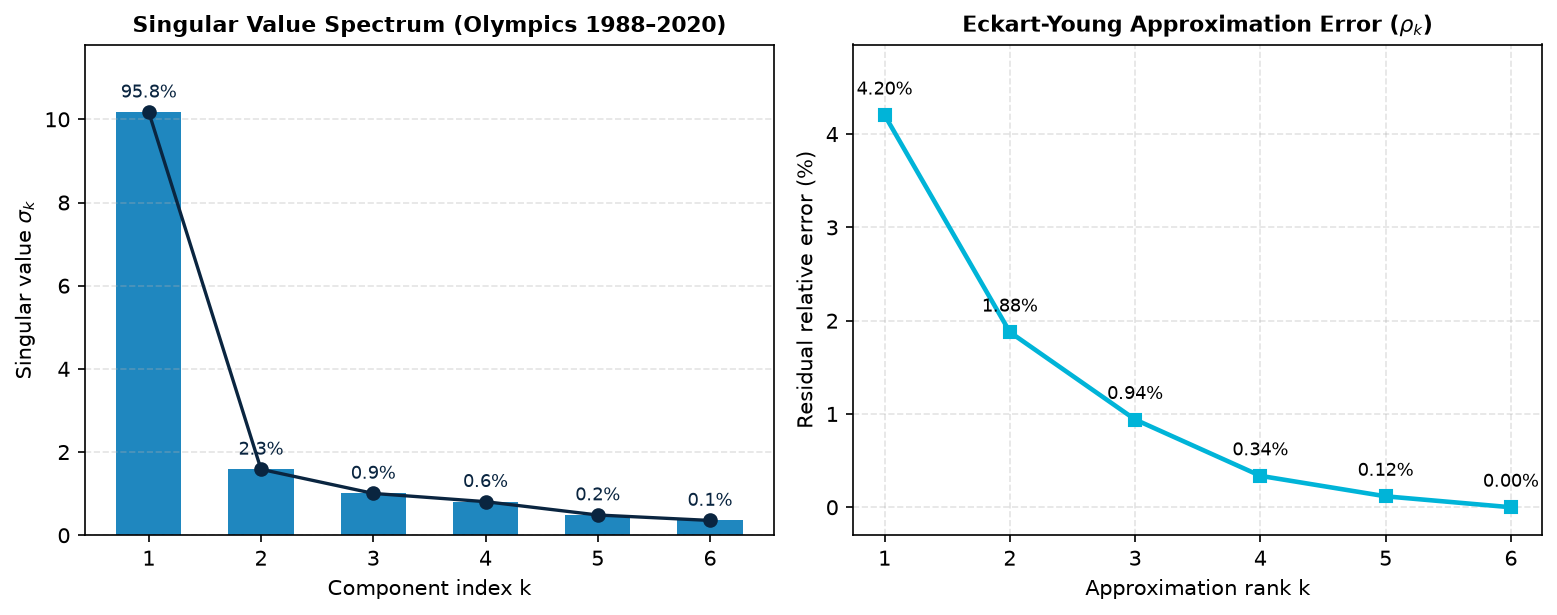
\includegraphics[width=0.95\textwidth]{figures/phase2_scree_eckart_young.png}
    \caption{Singular value spectrum (left) and Eckart--Young rank-$k$ approximation error $\rho_k$ (right) on the complete 1988--2020 Olympic finals matrix ($m=18$, $n=6$).}
    \label{fig:scree_eckart}
\end{figure}

Figure~\ref{fig:scree_eckart} shows a strongly dominated spectrum ($\sigma = [10.172, 1.585, 1.006, 0.807, 0.487, 0.356]$), where the first two principal components represent:
\begin{itemize}
    \item \textbf{PC1 (95.8\% of variance): overall historical progression.} PC1 loads almost equally across all six events ($v_1 = [-0.409, -0.413, -0.413, -0.394, -0.409, -0.411]$), measuring the global improvement in Olympic swimming times from 1988 to 2020 across every stroke and distance.

    \item \textbf{PC2 (2.33\% of variance): sprint vs.\ 400\,m contrast.} PC2 loads positively on the shorter events (\texttt{50m Free}: $+0.220$, \texttt{100m Free}: $+0.242$, \texttt{100m Fly}: $+0.248$, \texttt{200m IM}: $+0.237$) and strongly negatively on \texttt{400m Free} ($-0.874$), separating sprint evolution from mid-distance progression.
\end{itemize}
A rank-2 projection already preserves $98.12\%$ of total variance ($\rho_2 = 1.88\%$). However, the small last singular value ($\sigma_6 = 0.356$) leads to $\kappa_2(X) = 28.58$ and $\kappa_2(X^T X) = 816.86$. This high condition number confirms that Olympic events are tightly collinear, which will cause unregularized linear regression to suffer from variance inflation in Section~3.

\subsection{Swimmer Sprint Profiles (PCA Biplot)}

We next study individual athletes from the multi-event matrix across the four core sprint events around 100\,m Freestyle (\texttt{50m}, \texttt{100m}, \texttt{200m Free}, and \texttt{100m Fly}). Keeping swimmers with at least two recorded events gives $m=129$ athletes. After gender-wise standardization, missing entries are filled using iterative rank-2 SVD completion.

\begin{figure}[H]
    \centering
    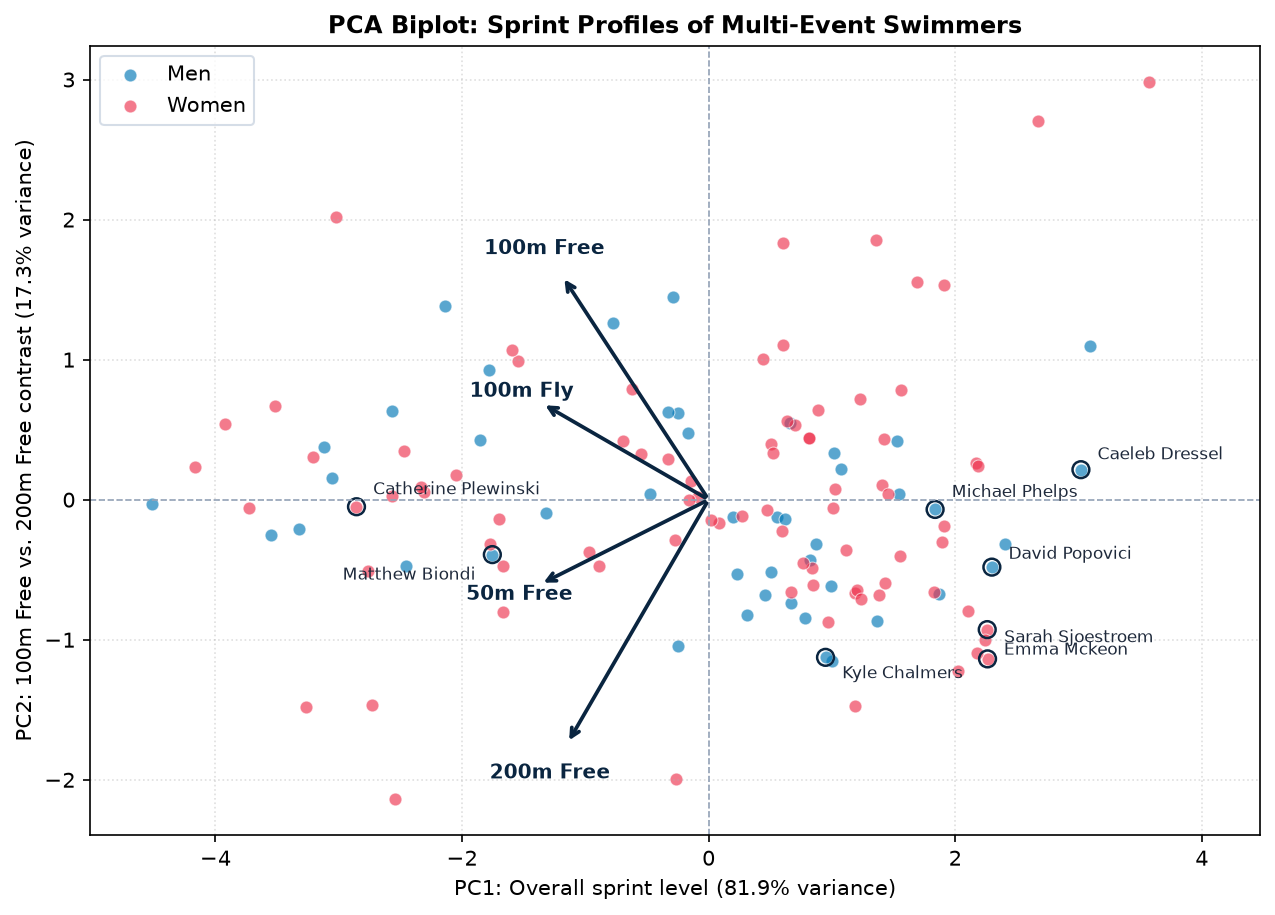
\includegraphics[width=0.86\textwidth]{figures/phase2_biplot_sprint.png}
    \caption{PCA biplot of $m=129$ versatile sprint swimmers ($n=4$ events, completed via rank-2 SVD). Faster swimmers appear on the right ($\text{PC1} > 0$), while event time arrows point left.}
    \label{fig:biplot_sprint}
\end{figure}

Figure~\ref{fig:biplot_sprint} projects the 129 swimmers onto the plane $(\text{PC1}, \text{PC2})$. Explicitly, the two components are:
\begin{align}
    \text{PC1} &= -0.540\,z_{50} - 0.468\,z_{100} - 0.453\,z_{200} - 0.534\,z_{100\text{Fly}}, \\
    \text{PC2} &= -0.239\,z_{50} + 0.630\,z_{100} - 0.687\,z_{200} + 0.272\,z_{100\text{Fly}}.
\end{align}
Their sporting meaning is clear:
\begin{itemize}
    \item \textbf{PC1 (81.9\% of variance): overall sprint level.} All four event times enter PC1 with negative weights of similar magnitude. Since lower times correspond to negative standardized values $z$, faster swimmers obtain positive PC1 scores and sit on the right of the biplot (e.g.\ Caeleb Dressel at $\text{PC1}=+3.02$, David Popovici at $+2.30$, Sarah Sjoestroem and Emma McKeon at $+2.26$, Michael Phelps at $+1.84$), whereas earlier-era or slower swimmers lie on the left.

    \item \textbf{PC2 (17.3\% of variance): 100\,m vs.\ 200\,m balance.} PC2 opposes \texttt{100m Free} ($+0.630$) and \texttt{100m Fly} ($+0.272$) against \texttt{200m Free} ($-0.687$) and \texttt{50m Free} ($-0.239$). Because faster times are negative after standardization, negative PC2 scores identify swimmers who are relatively faster in the 100\,m than in the 200\,m Freestyle (such as Kyle Chalmers at $\text{PC2}=-1.13$ with 47.08\,s vs.\ 105.48\,s, or Sarah Sjoestroem at $-1.14$), whereas balanced 100\,m/200\,m performers like Michael Phelps ($\text{PC2}=-0.07$, 47.51\,s vs.\ 102.96\,s) sit near zero.
\end{itemize}

\noindent \textbf{Methodological note:} iterative rank-2 SVD completion mechanically concentrates $99.2\%$ of total variance onto PC1 and PC2. For this reason, the biplot is best read as a clean 2D map of swimmer profiles, while the complete Olympic matrix (Sec.~2.2) remains our unbiased spectral reference.

% ============================================================
% REFERENCES
% ============================================================
\clearpage
\phantomsection
\addcontentsline{toc}{section}{References}
\begin{thebibliography}{9}

\bibitem{kaggle_top200}
\texttt{romaniandatatribe},
\textit{Swimming: Top In The World In Each Category},
Kaggle dataset, World Aquatics top-200 historical long-course times (1980--2022).
Available at: \url{https://www.kaggle.com/datasets/romaniandatatribe/swimming-top-in-the-world-in-each-category}.

\bibitem{kaggle_olympics}
\texttt{datasciencedonut},
\textit{Olympic Swimming 1912 to 2020},
Kaggle dataset, historical Olympic Games swimming event results.
Available at: \url{https://www.kaggle.com/datasets/datasciencedonut/olympic-swimming-1912-to-2020}.

\bibitem{hastie2009}
T.~Hastie, R.~Tibshirani, and J.~Friedman,
\textit{The Elements of Statistical Learning: Data Mining, Inference, and Prediction},
2nd ed., Springer Series in Statistics, Springer, 2009.
DOI: \url{https://doi.org/10.1007/b94608}.
Official open-access edition: \url{https://hastie.su.domains/ElemStatLearn/}.

\bibitem{deisenroth2020}
M.~P.~Deisenroth, A.~A.~Faisal, and C.~S.~Ong,
\textit{Mathematics for Machine Learning},
Cambridge University Press, 2020 (Secs.~4.5--4.6: SVD and Matrix Approximation).
ISBN 978-1-108-45514-5.
Official open-access PDF: \url{https://mml-book.github.io/}.

\bibitem{wasserman2004}
L.~Wasserman,
\textit{All of Statistics: A Concise Course in Statistical Inference},
Springer Texts in Statistics, Springer, 2004.
ISBN 978-0-387-40272-7, DOI: \url{https://doi.org/10.1007/978-0-387-21736-9}.
Official book resource page: \url{https://www.stat.cmu.edu/~larry/all-of-statistics/}.

\end{thebibliography}

\end{document}
